\documentclass[lettersize,journal]{IEEEtran}
\usepackage{amsmath,amsfonts}
\usepackage{algorithmic}
\usepackage{algorithm}
\usepackage{array}
\usepackage[caption=false,font=normalsize,labelfont=sf,textfont=sf]{subfig}
\usepackage{textcomp}
\usepackage{stfloats}
\usepackage{url}
\usepackage{verbatim}
\usepackage{graphicx}
\usepackage{cite}
\usepackage{tikz}
\usetikzlibrary{arrows.meta,fit,backgrounds}
\usepackage{booktabs}
\usepackage{placeins}
\hyphenation{op-tical net-works semi-conduc-tor IEEE-Xplore}

\begin{document}

\title{Midterm Report: An IoT System for Real-time Human Activity Recognition}

\author{Tianchen Liu$^{*}$, Juntao Hu$^{*}$
\thanks{$^*$ equal contribution.}
\thanks{Progress report, 28 October 2026. The final presentation is on 20 November 2026.}}

\maketitle

\begin{abstract}
This report records the midterm state of the smartphone--laptop activity
system proposed for IERG5230. A 4-bit SmolVLM-256M in the phone browser
writes a short action phrase and a minimum token probability. A frame
close to the previous one keeps the ongoing phrase and skips that model.
The picture stays on the phone when the new phrase is confident and still
matches the ongoing action. A confident mismatch must occur on two frames
before the buffered frames are uploaded. Low token confidence uploads on
the current frame. Qwen3.5-2B on the laptop then writes its own phrase.
The phrases are compared by text-encoder cosine similarity, not by a closed
caption bank. On 60 still images the cosine matcher scores 38/60 for
SmolVLM and 40/60 for Qwen. Replaying the live rule on three frames per
clip scores 1640/3783 on UCF101 and 660/1530 on HMDB51, below a single
Qwen pass over the same frames. The latency predictor, the dynamic uplink
budget, and the multi-client scheduler are specified and are not running
yet.
\end{abstract}

\section{Introduction}

An interactive system has to name the activity while the person is still
moving. A closed label such as ``sitting'' is too coarse for that response.
Sitting still, sitting and looking at a phone, and sitting and waving call
for different responses, yet a small label set collapses them into one
class. The system therefore describes the activity with a short English
phrase. A strong vision-language model can write that phrase, but running
it on every captured frame is too expensive for a phone, and uploading
every frame makes the user wait on the uplink.

The design splits the work. SmolVLM-256M-Instruct runs in the phone browser
and writes the phrase before any picture leaves the device
\cite{marafioti2025smolvlm}. The confidence of the phrase is the smallest
probability among the newly generated tokens. The JPEG stays on the phone
when this confidence is high and the phrase still agrees with the action
already on screen. Otherwise the phone uploads the last few frames. A
laptop on the same Wi-Fi network runs Qwen3.5-2B, writes its own phrase,
and the screen keeps or replaces the ongoing phrase according to the cosine
similarity of the two texts.

Two choices in the proposal have been changed because they fought that
goal. The proposal kept a fixed sentence bank and let CLIP retrieve one
bank sentence for the phone text and another for the picture. The screen
then showed the bank sentence. The running system keeps the model's own
phrase. The bank is used only when a free phrase must be scored against the
15 classes of the still-image evaluation. The proposal also planned a
compute-aware upload scheduler. That scheduler is the networking half of
the project. This midterm finishes the sentence-and-check path, including a
causal check over the last few frames, and states the scheduler work that
is still ahead.

The sentence path now has two extra gates in front of that upload. A live
frame is reduced to a \(32\times 32\) grayscale image. When an action is
already on screen, the leave count is zero, and the mean absolute
difference from the previous frame is below 10, the phone keeps the phrase
and does not run SmolVLM. A confident phrase that leaves the action is
held for one frame. The buffered frames go to Qwen only on a second
mismatch. A missing or low token probability does not wait. On a 60-image
sample the text-encoder matcher scores 38/60 for the phone model and 40/60
for Qwen. The same live rule, replayed on three frames from each test
clip, scores 1640/3783 on UCF101 and 660/1530 on HMDB51. A single Qwen
pass over those three frames scores 1785/3783 and 812/1530.

The rest of this report is organized as follows.
Section~\ref{sec:literature} places the prototype among activity
recognizers, vision-language models, and edge offloading systems.
Section~\ref{sec:objectives} states the objectives and which of them this
midterm meets.
Section~\ref{sec:design} gives the keep rule, the three-frame check, and
the upload control that is still to be built.
Section~\ref{sec:implementation} describes the browser client and the
laptop server.
Section~\ref{sec:evaluation} reports the still-image measurement and the
three-frame replay on UCF101 and HMDB51.
Section~\ref{sec:conclusion} states what the measurement supports and what
remains before the presentation on 20 November 2026.

\section{Literature Study}
\label{sec:literature}

\subsection{Activity labels and free phrases}

Activity recognizers take RGB, skeleton, IMU, radar, or Wi-Fi, and usually
return one label from a closed set. An open-set model can reject an unknown
action. It still does not describe that action. An open-vocabulary model
can match a clip to a class name while the action is still going on.
Free-form captions also exist. OV-HAR turns a sensor window into a sentence
\cite{ray2025ovhar}, and OpenHOUSE calls a vision-language model for a
free-form description of streaming video \cite{kang2025openhouse}. Both are
evaluated on recorded data, not on a live phone link.

Recent video benchmarks such as Kinetics-400 are clips of about ten
seconds. A single decoded frame, or three frames a second apart, does not
support a claim on that benchmark. Online action detection reads only past
frames and emits a label at every time step. The prototype is causal, in
that it never reads a frame that has not been captured, but it updates only
as fast as the phone model finishes one still image. The missing piece in
the cited caption systems is a sentence produced on the phone, before any
picture is uploaded, while the person is still moving.

\subsection{Retrieval and generative vision-language models}

CLIP retrieves a sentence from a fixed bank by cosine similarity between an
image embedding, or a text embedding, and the bank
\cite{radford2021learning}. It does not write a new sentence. That
retrieval was the checker in the proposal: the phone phrase and the
uploaded picture were each mapped to one bank sentence, and the screen
showed the bank sentence. A generative vision-language model writes the
sentence token by token, and accuracy follows model size. Qwen2-VL scales
this family up to 72B parameters \cite{wang2024qwen2vl}. Models that can
sit on a phone also exist. MiniCPM-V is in the 2B--8B range
\cite{yao2024minicpm}, and SmolVLM-256M fits in under 1~GB
\cite{marafioti2025smolvlm}. Published scores for these models cover
documents, charts, and general questions, not fine differences between
similar activities.

A small generative model can therefore write the sentence on the phone. It
does not, by itself, say which of those sentences are safe to leave on the
screen. The checker in this report follows the text half of the CLIP
comparison and not the image encoder. Both the phone phrase and the laptop
phrase are encoded by a text embedding model, and the score is their cosine
\cite{xiao2024cpack}. Mapping either phrase onto a class sentence for the
still-image evaluation uses the same score:
\begin{equation}
\label{eq:class}
c
=
\arg\max_{c\in\mathcal{C}}
\cos\big(f_T(s), e_c\big).
\end{equation}
The live screen does not apply \eqref{eq:class}. It shows $s$ itself.

\subsection{Client--server collaboration}

Neurosurgeon profiles network layers and chooses where to split them, so
the server receives image features and the user waits for that transfer
\cite{kang2017neurosurgeon}. Speculative decoding splits the work by
tokens: a small model drafts, a large model verifies, and the server still
reads the picture \cite{leviathan2023fast,chen2023accelerating}. Later
edge variants keep the same split
\cite{jia2026covspec,venkatesha2025fast}. edgeVLM answers on the device at
once and reuses a late cloud caption as context for later frames, rather
than as the result of the frame that is on screen now
\cite{qian2025edgevlm}. EdgeBoost uploads an input only when the local
confidence is low. On image classification this removes about 20--55\% of
the communication of a cloud-only run, and the cloud still returns a class
label \cite{said2024edgeboost}.

What these systems return is a class, a feature tensor, or a caption that
arrives after the frame has moved on. The prototype shows an activity
phrase as soon as the phone finishes, and it sends the picture only when
that phrase is unsafe relative to the action already on screen.

\subsection{Communication after the phrase exists}

A proportional-fair scheduler and an L4S queue assign service to packets
that have already been formed. They do not look at how long the laptop will
spend on the picture after it arrives
\cite{jalali2000data,briscoe2023l4s}. Semantic communication scores a
transmission by task success rather than by throughput, but the payload is
still a feature tensor \cite{xie2021deep}. Offloading chooses local or
remote execution, and adaptive streaming changes how many bytes are sent.
After the sentence has already been written, these mechanisms still leave
open whether the picture should follow, how large that picture should be,
and which phone should be checked first.

The proposal takes that last decision. Token confidence decides whether the
JPEG is uploaded. JPEG quality and resolution decide its size. For every
upload, the predicted edge latency sets the uplink deadline, and an
application-layer scheduler serves the earliest deadline first. The running
prototype implements the confidence decision and a fixed JPEG size. The
predictor and the scheduler are specified in Section~\ref{sec:design} and
are not in the code yet.

\section{Objectives}
\label{sec:objectives}

The project has an information-processing half and a networking half. The
information-processing half is the phrase on the phone and the check on the
laptop. The networking half is the decision of when that check is allowed
to occupy the uplink. Table~\ref{tab:objectives} lists the objectives and
the midterm status of each one.

\begin{table}[t]
\caption{Objectives and midterm status}
\label{tab:objectives}
\centering
\footnotesize
\begin{tabular}{p{0.72\columnwidth}c}
\toprule
Objective & Status \\
\midrule
Write an English action phrase on the phone before any picture is uploaded &
Done \\
Keep the picture on the phone when the phrase is confident and still matches the ongoing action &
Done \\
Let the laptop write its own phrase and compare the two phrases by text cosine &
Done \\
Check a short causal clip of the last three frames when the local test fails &
Done \\
Score free phrases on 60 still images and on three-frame UCF101 and HMDB51 clips &
Done \\
Predict checker latency, set a per-frame uplink budget, and schedule several phones &
Planned \\
\bottomrule
\end{tabular}
\end{table}

The first objective is a phrase, not a class identifier. The phone model
must finish generation, and the page must show the phrase, without waiting
for the laptop. The confidence attached to that phrase is the minimum
probability of the new tokens, so a single uncertain token can force a
check.

The second objective is the upload gate. A high confidence is not enough on
its own once an action is already on screen. The new phrase must also stay
close to that action. The picture is the payload that this gate can
suppress. The phrase itself may still be sent, because the text encoder
runs on the laptop.

The third objective replaces the proposal's bank caption. The laptop model
writes a free phrase. Agreement is the cosine of the two phrase embeddings.
The screen keeps the model's words. A class sentence is introduced only in
the evaluation, where a free phrase has to be counted against a label.

The fourth objective keeps the check causal and short. The phone reads the
newest frame. The laptop, and only the laptop, may read the last three
frames, captured about one second apart and uploaded in time order. The
system does not wait for a future frame, and it does not claim a
ten-second clip.

The fifth objective is a measurement that can be repeated. The models are
not trained on either sample. The still-image check scores one free phrase
against 15 class sentences. The video check replays the live rule on three
frames from each clip in the UCF101 recognition test list and the HMDB51
test list. Those frames are taken around the middle of the clip. The
replay therefore scores the gate, the quiet skip, and the phrase, and it
does not score the start or the end of an action.

The sixth objective is unchanged from the proposal and is not met at this
midterm. Before an upload, the laptop should predict how long the checker
will take, subtract that time from the confirmation deadline, and turn the
remainder into an uplink budget. When several phones ask for a check at
once, the earliest uplink deadline should go first. The November work is
to collect the traces, train the predictor, and compare that rule with
round-robin and with a static budget.

\section{Design}
\label{sec:design}

Figure~\ref{fig:framework} is the path that is running. A quiet frame keeps
the phrase and skips the phone model. Otherwise the phone writes and shows
a phrase before any picture leaves the device. The sentence crosses the
Wi-Fi link for a semantic check. The JPEG follows immediately when token
confidence is low, and only on a second frame when a confident phrase has
left the ongoing action. The latency predictor and the upload scheduler
are not on this figure.

\subsection{Local phrase and confidence}

SmolVLM-256M-Instruct runs in the phone browser at 4-bit. For a frame
$x_i$ it writes a phrase $s_i$ and a probability $p_{i,t}$ for each new
token. The confidence is the weakest of those probabilities,
\begin{equation}
\label{eq:kappa}
\kappa_i = \min_t p_{i,t}.
\end{equation}
The phrase is shown when local generation finishes. It does not wait for
the laptop. An empty phrase has confidence missing and is treated as
unsafe. The phone prompt asks for a short action phrase and nothing else,
so the later cosine compares two phrases of the same kind.

\subsection{When the picture stays on the phone}

Let $a$ be the phrase of the action that is already on screen, and let
$\tau_{\mathrm{u}}$ and $\tau_{\mathrm{s}}$ be the confidence and cosine
thresholds. The JPEG stays on the phone when the local phrase is confident
and still close to that action:
\begin{equation}
\label{eq:keep}
\kappa_i \ge \tau_{\mathrm{u}}
\quad\text{and}\quad
\cos\big(f_T(s_i), f_T(a)\big) \ge \tau_{\mathrm{s}}.
\end{equation}
The defaults in the prototype are $\tau_{\mathrm{u}}=0.5$ and
$\tau_{\mathrm{s}}=0.70$. The text encoder $f_T$ is
\texttt{bge-small-en-v1.5}, running on the laptop CPU so the GPU remains
available for Qwen \cite{xiao2024cpack}. An empty phrase scores 0. The
first confident phrase of a session starts the action. There is no $a$ yet,
so only the confidence test applies, and the picture is not uploaded.

The cosine in \eqref{eq:keep} is computed on the laptop. A confident live
frame therefore still sends the phrase. It does not send the JPEG. One
failure of that cosine test increments a leave count and keeps $a$. The
buffered frames are uploaded only when the count reaches 2. The count
returns to 0 when the phrases match, when Qwen returns a decision, and at
the start of a new action. One-shot capture and a file upload do not use
the action state, the leave count, or the quiet-frame test. They compare
$s_i$ with the laptop phrase only.

\subsection{Quiet frames}

Before SmolVLM runs, the live page scales the current JPEG to a
\(32\times 32\) grayscale image \(g_i\). The distance from the previous
live frame is the mean absolute difference
\begin{equation}
\label{eq:mad}
d_i
=
\frac{1}{1024}
\sum_{u=1}^{32}
\sum_{v=1}^{32}
\left|g_i(u,v)-g_{i-1}(u,v)\right|.
\end{equation}
SmolVLM is skipped, and \(a\) stays on screen, when an action is already
set, the leave count is 0, and \(d_i<10\). A frame that is waiting for a
second mismatch is not treated as quiet, so a pending leave is not erased
by a small pixel change. The first frame of a session has no previous
image and always reaches the model. The same threshold and the same
\(32\times 32\) signature are used by the video replay.

\begin{figure*}[t]
\centering
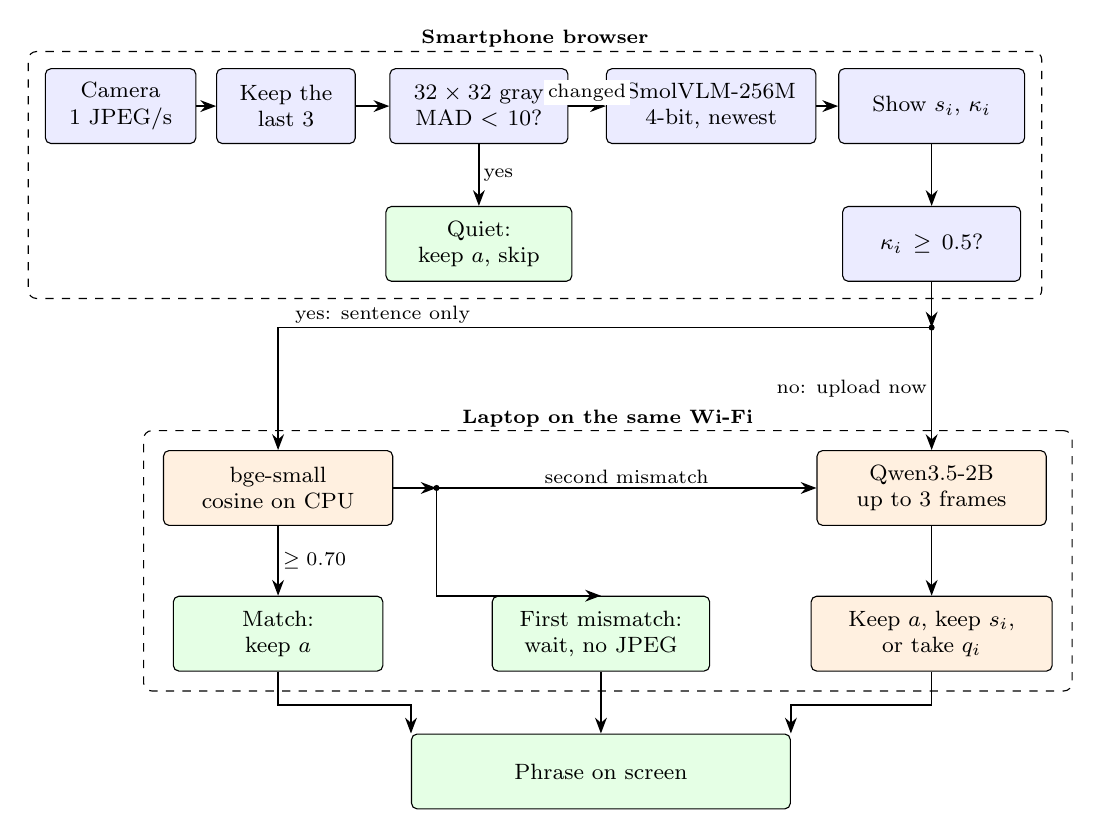
\begin{tikzpicture}[
    font=\footnotesize,
    >=Stealth,
    block/.style={
      draw, rounded corners=2pt, align=center,
      inner sep=3pt, fill=white, minimum height=9.5mm
    },
    phone/.style={block, fill=blue!8},
    edge/.style={block, fill=orange!12},
    result/.style={block, fill=green!10},
    arr/.style={->, semithick},
    tag/.style={font=\scriptsize, inner sep=1.4pt, align=center, fill=white}
  ]
  \node[phone, text width=1.7cm] (cam) at (1.05,0) {Camera\\1 JPEG/s};
  \node[phone, text width=1.55cm] (buf) at (3.15,0) {Keep the\\last 3};
  \node[phone, text width=2.05cm] (mad) at (5.6,0) {$32\times 32$ gray\\MAD $<10$?};
  \node[phone, text width=2.45cm] (smol) at (8.55,0) {SmolVLM-256M\\4-bit, newest};
  \node[phone, text width=2.15cm] (show) at (11.35,0) {Show $s_i$, $\kappa_i$};
  \node[result, text width=2.15cm] (skip) at (5.6,-1.75) {Quiet:\\keep $a$, skip};
  \node[phone, text width=2.05cm] (gate) at (11.35,-1.75) {$\kappa_i\ge 0.5$?};

  \node[edge, text width=2.7cm] (bge) at (3.05,-4.85)
    {bge-small\\cosine on CPU};
  \node[result, text width=2.45cm] (keep) at (3.05,-6.7) {Match:\\keep $a$};
  \node[result, text width=2.55cm] (wait) at (7.15,-6.7)
    {First mismatch:\\wait, no JPEG};
  \node[edge, text width=2.7cm] (qwen) at (11.35,-4.85)
    {Qwen3.5-2B\\up to 3 frames};
  \node[edge, text width=2.85cm] (fuse) at (11.35,-6.7)
    {Keep $a$, keep $s_i$,\\or take $q_i$};
  \node[result, text width=4.6cm] (final) at (7.15,-8.45)
    {Phrase on screen};

  \draw[arr] (cam) -- (buf);
  \draw[arr] (buf) -- (mad);
  \draw[arr] (mad) -- node[tag, above] {changed} (smol);
  \draw[arr] (smol) -- (show);
  \draw[arr] (show) -- (gate);
  \draw[arr] (mad) -- node[tag, right] {yes} (skip);

  \draw[arr] (gate.south) -- ++(0,-0.58) coordinate (split);
  \fill (split) circle[radius=1.1pt];
  \draw[arr] (split) -|
    node[tag, pos=0.42, above] {yes: sentence only}
    (bge.north);
  \draw[arr] (split) --
    node[tag, left] {no: upload now}
    (qwen.north);

  \draw[arr] (bge) -- node[tag, right] {$\ge 0.70$} (keep);
  \draw[arr] (bge.east) -- ++(0.55,0) coordinate (miss);
  \fill (miss) circle[radius=1.1pt];
  \draw[arr] (miss) --
    node[tag, above] {second mismatch}
    (qwen.west);
  \draw[arr] (miss) |- (wait.north);
  \draw[arr] (qwen) -- (fuse);

  \draw[arr] (keep.south) -- ++(0,-0.42) -| (final.north west);
  \draw[arr] (fuse.south) -- ++(0,-0.42) -| (final.north east);
  \draw[arr] (wait.south) -- (final.north);

  \begin{scope}[on background layer]
    \node[draw, dashed, rounded corners=3pt, inner sep=6pt,
          fit=(cam)(buf)(mad)(smol)(show)(skip)(gate)] (phonebox) {};
    \node[draw, dashed, rounded corners=3pt, inner sep=7pt,
          fit=(bge)(keep)(wait)(qwen)(fuse)] (lapbox) {};
  \end{scope}
  \node[font=\scriptsize\bfseries, anchor=south, inner sep=1pt]
    at (phonebox.north) {Smartphone browser};
  \node[font=\scriptsize\bfseries, anchor=south, inner sep=1pt]
    at (lapbox.north) {Laptop on the same Wi-Fi};
\end{tikzpicture}
\caption{Live framework. A quiet frame, measured by a $32\times 32$
grayscale mean absolute difference below 10, keeps the ongoing phrase and
skips SmolVLM. Otherwise the phone shows $s_i$ at once. Low token
confidence uploads the buffered frames immediately. A confident phrase
sends the sentence only. The text encoder keeps the action when the
sentence is still close. The first mismatch waits. The second mismatch
uploads, and Qwen's phrase is kept only when it agrees with neither $a$
nor $s_i$. The first confident phrase of a session starts $a$ with no
cosine test.}
\label{fig:framework}
\end{figure*}


\subsection{Three-frame check}

Live mode stores one JPEG per second and keeps the last three. SmolVLM is
invoked on the newest frame only, and only when \eqref{eq:mad} does not
skip it. While it runs, newer captures replace the buffer and are not
queued behind the frame already in inference. The upload uses those frames
in time order. It happens on the current frame when $\kappa_i$ is missing
or below $\tau_{\mathrm{u}}$. It happens on a confident frame only after
two cosine failures. Qwen3.5-2B then writes one phrase $q_i$ for the frames
it receives. The prompt states that the frames are about one second apart.
A single uploaded frame uses the same short-action prompt as the phone.

The ongoing phrase $a$ is kept when $q_i$ is close to it. Otherwise the
screen uses $s_i$ when $q_i$ is close to $s_i$ or when $q_i$ is empty, and
uses $q_i$ when the two phrases disagree:
\begin{equation}
\label{eq:fuse}
a^{+} =
\begin{cases}
a & \text{if } a\neq\emptyset \text{ and } \cos(f_T(q_i),f_T(a))\ge\tau_{\mathrm{s}},\\
s_i & \text{if } q_i=\emptyset \text{ or } \cos(f_T(s_i),f_T(q_i))\ge\tau_{\mathrm{s}},\\
q_i & \text{otherwise.}
\end{cases}
\end{equation}
A kept action does not reset its start time. A replaced action starts at
the newest frame. Algorithm~\ref{alg:live} is the live procedure.

\begin{algorithm}[t]
\caption{Live phrase with a quiet skip and a two-frame leave}
\label{alg:live}
\begin{algorithmic}[1]
\STATE Keep the last three JPEGs, one captured per second.
\STATE Compute \(d_i\) in \eqref{eq:mad}. Let \(\ell\) be the leave count.
\IF{\(a\) is set and \(\ell=0\) and \(d_i<10\)}
    \STATE Keep \(a\) and skip SmolVLM.
\ELSE
    \STATE Run 4-bit SmolVLM on the newest frame and display \(s_i\).
    \STATE \(\kappa_i\leftarrow\min_t p_{i,t}\).
    \IF{\(\kappa_i<\tau_{\mathrm{u}}\) or \(\kappa_i\) is missing}
        \STATE Upload the buffered frames, oldest first.
    \ELSIF{\(a\) is unset}
        \STATE Start \(a\) from \(s_i\). Do not upload.
    \ELSIF{\(\cos(f_T(s_i),f_T(a))\ge\tau_{\mathrm{s}}\)}
        \STATE Keep \(a\) and set \(\ell\leftarrow 0\).
    \ELSE
        \STATE \(\ell\leftarrow\ell+1\).
        \IF{\(\ell<2\)}
            \STATE Keep \(a\). Do not upload.
        \ELSE
            \STATE Upload the buffered frames, oldest first.
        \ENDIF
    \ENDIF
\ENDIF
\IF{frames were uploaded}
    \STATE Qwen writes \(q_i\) and apply \eqref{eq:fuse}.
    \STATE Set \(\ell\leftarrow 0\).
\ENDIF
\end{algorithmic}
\end{algorithm}

The phone model still reads one still image. Three frames are joint input
only for Qwen, and only after the local check fails. The vision encoder of
SmolVLM resizes its input and emits a fixed image-token sequence, so
stitching the three frames into one JPEG would shrink each frame instead of
adding time. The update period is the phone generation time. On the
development phone with WebGPU that time is under three seconds, so actions
shorter than the period can fall between updates. This is not per-frame
online detection and not a Kinetics evaluation.

\subsection{Upload control still to be built}

The sentence that appears first is local,
$T_i^{\mathrm{draft}}=T_i^{\mathrm{local}}$,
where $T_i^{\mathrm{local}}$ is the SmolVLM time on the phone. A frame that
fails \eqref{eq:keep} also waits for a checked phrase. Its confirmation
delay is
\begin{equation}
\label{eq:conf}
T_i^{\mathrm{conf}}
=
T_i^{\mathrm{wait}}
+
T_i^{\mathrm{up}}
+
T_i^{\mathrm{edge}}
+
T_i^{\mathrm{down}},
\end{equation}
where $T_i^{\mathrm{wait}}$ is the time until an upload grant,
$T_i^{\mathrm{up}}$ is the JPEG upload, $T_i^{\mathrm{edge}}$ is the checker,
and $T_i^{\mathrm{down}}$ is the return of a short result. The request meets
its deadline when $T_i^{\mathrm{conf}}\le D_i^{\mathrm{conf}}$.

Checker time is not a constant. The predictor planned for November reads
\begin{equation}
\mathbf{z}_i
=
\left[
L_i,\;
U_i^{\mathrm{CPU}},\;
T_{i-1}^{\mathrm{edge}}
\right],
\end{equation}
with $L_i$ the JPEG size in bytes, $U_i^{\mathrm{CPU}}$ the server load at
the request, and $T_{i-1}^{\mathrm{edge}}$ the previous checking time. A
small network $g_\theta$ predicts $\hat T_i^{\mathrm{edge}}=g_\theta(\mathbf{z}_i)$
before the JPEG is uploaded. The remaining uplink budget is
\begin{equation}
\label{eq:budget}
B_i^{\mathrm{up}}
=
\left[
D_i^{\mathrm{conf}}
-
\hat T_i^{\mathrm{edge}}
-
\hat T_i^{\mathrm{down}}
-
M
\right]^+,
\end{equation}
and the uplink deadline is $d_i^{\mathrm{up}}=a_i+B_i^{\mathrm{up}}$ from
the arrival time $a_i$. The scheduler serves
\begin{equation}
i^\star=\arg\min_{i\in\mathcal{Q}} d_i^{\mathrm{up}}.
\end{equation}
A long predicted edge time leaves less room for the upload, so that request
gets an earlier deadline. None of $g_\theta$, $B_i^{\mathrm{up}}$, or the
queue $\mathcal{Q}$ is in the prototype. The phone does not send a planned
JPEG size or a confirmation deadline, and the laptop does not order
uploads.

\section{Implementation}
\label{sec:implementation}

\subsection{Phone browser}

The client is a smartphone browser. The page is served by the laptop.
SmolVLM-256M-Instruct runs in a Web Worker through Transformers.js~3.7.1.
The vision encoder and the decoder use 4-bit weights. Token embeddings stay
in 16-bit. WebGPU is selected when the browser exposes an adapter. If that
adapter supports \texttt{shader-f16}, the 4-bit weights are stored in the
16-bit WebGPU variant. Otherwise the worker uses the plain 4-bit variant.
If WebGPU fails to start the model, the worker loads the same 4-bit weights
on WASM. WASM uses up to four threads when the page is cross-origin
isolated and the device is not an iPhone. The laptop sends
\texttt{Cross-Origin-Opener-Policy} and
\texttt{Cross-Origin-Embedder-Policy} so a desktop browser can take that
threaded fallback. On the development phone, WebGPU brings one-frame
generation under three seconds.

The generation call in the browser does not return a score tensor. The
worker therefore installs a logits processor, reads the logits of each new
token, and turns the maximum logit into a probability with a log-sum-exp.
The confidence reported to the page is the minimum of those probabilities,
which is $\kappa_i$ in \eqref{eq:kappa}. Generation is greedy and stops at
16 new tokens. The prompt is ``What is the person doing? Answer with only a
short action phrase.'' The vision encoder resizes its input and emits a
fixed image-token sequence, so the worker does not split the image into
tiles, and it scales the longest side to 512 before inference. A smaller
JPEG would be scaled back up inside the encoder.

The camera path stores one JPEG per second at quality 0.72, longest side
512, and keeps three blobs. A front camera preview is mirrored. The blob
that enters the model is mirrored back so the encoder sees an unmirrored
frame. While a phrase is being generated, the capture clock continues and
the buffer keeps only the newest three frames. The next inference starts
from the newest frame after the current call returns. Before that call,
the page draws the frame onto a \(32\times 32\) canvas, converts it to
grayscale, and compares it with the previous live frame by
\eqref{eq:mad}. The page reads the threshold 10 and the leave limit 2 from
the server health check, which returns the constants in the shared policy
module. One-shot capture and a file chosen by the user send at most one
image and do not update the ongoing action.

\subsection{Laptop checker}

The laptop serves the page with FastAPI and loads Qwen3.5-2B in bfloat16 on
an RTX 5070 Laptop GPU. The phrase encoder,
\texttt{bge-small-en-v1.5}, is loaded on the CPU. Mean pooling over the
masked last hidden state, followed by $\ell_2$ normalization, produces the
vectors whose cosine is $\tau_{\mathrm{s}}$. One still image takes a few
hundred milliseconds after the weights are resident. A spot check with two
frames took 1.4 seconds. Qwen generation is also greedy, with at most 32
new tokens. Thinking mode is turned off. The image processor is capped at
$28\times 28\times 256$ pixels, and each uploaded frame is again limited to
a longest side of 512. A lock admits one Qwen call at a time.

The check endpoint receives the phone phrase, the ongoing phrase, and zero
to three JPEGs. With no JPEG it only compares the two phrases. A cosine of
at least 0.70 keeps the ongoing phrase and tells the phone not to upload.
With one or more JPEGs the server runs Qwen. The single-frame prompt
matches the phone. The multi-frame prompt adds that the images are in time
order and about one second apart. The reply is one of four outcomes. The
ongoing phrase is held when Qwen stays close to it. The phone phrase is
confirmed when Qwen stays close to the phone and not to the ongoing action.
The phone phrase is kept when Qwen returns an empty string. Otherwise the
screen takes Qwen's phrase. The certificate is reissued for the current
LAN address at every server start, so the phone can open the camera over
HTTPS. This path does not change the Wi-Fi MAC or the access point.

\subsection{Evaluation harness and division of work}

The still-image harness loads the labeled train split of the Bingsu human
action set, draws a stratified sample, and writes one phrase per image with
the same short-action prompt. Cached phrases can be matched again without
regenerating them. The class sentences are fixed English lines of the form
``a person is running''. The predicted class is \eqref{eq:class}. The video
harness takes three frames from each clip, caches a SmolVLM phrase per
frame and a Qwen phrase for each prefix length, and replays the quiet skip,
the leave count, and the fusion rule in the same policy module the server
uses. The phone worker is not part of either harness. Both load SmolVLM in
float32 on CUDA, so those SmolVLM times are not the 4-bit browser times.

Both members integrate the demo, the evaluation, and the report. Juntao Hu
is responsible for the local model, the acceptance rule, the laptop
checker, and the caption-quality evaluation. That path is running. Tianchen
Liu is responsible for the latency predictor, the dynamic uplink budget,
the upload scheduler, and the multi-client simulation. That path has not
been implemented.

\section{Evaluation}
\label{sec:evaluation}

\subsection{Protocol}

The still-image check uses the Human Action Recognition set released by
Bingsu. The published test split has placeholder labels, so the sample is
drawn from the labeled train split: 15 classes, 4 images per class, seed 0,
60 images. The models are not trained on it. Each model sees one image and
writes a free phrase with the same short-action prompt. The predicted class
is the class sentence with the highest text-encoder cosine. An earlier
matcher based on character overlap, with a bonus when the class name
appeared in the phrase, is kept only as a reference.

This protocol scores \eqref{eq:class}. It does not score
\eqref{eq:keep}, \eqref{eq:mad}, or \eqref{eq:fuse}. There is no ongoing
action across the 60 images, and Qwen sees one frame rather than three.
A phrase can describe the picture in ordinary English and still miss the
class, because the class sentence is a single canonical line. ``Typing''
sits near both texting and using a laptop. The cosine can prefer either
neighbor.

\subsection{Phrase-to-class accuracy}

\begin{table}[t]
\caption{Phrase-to-class accuracy on 60 still images.}
\label{tab:still}
\centering
\begin{tabular}{lcc}
\toprule
Matcher & SmolVLM & Qwen \\
\midrule
Character overlap & 27/60 & 30/60 \\
Text-encoder cosine & 38/60 & 40/60 \\
\bottomrule
\end{tabular}
\end{table}

Table~\ref{tab:still} shows that the text encoder recovers paraphrases that
character overlap misses. ``Riding bike'' matches cycling, and ``Drinking
wine'' matches drinking, without the class name having to appear as a
substring. The gain is 11 images for SmolVLM and 10 images for Qwen. Qwen
is ahead of SmolVLM by two images under the cosine matcher. On this sample
the larger model is not a large gain once both models are allowed to speak
in their own words and a text encoder absorbs the wording.

Table~\ref{tab:class} breaks the cosine score down by class. Both models
are correct on all four running images and fail most texting and
laptop images. SmolVLM is correct on all four calling images. Qwen writes
``talking'' or ``using a phone'' on several of those images, and the cosine
then prefers texting or calling inconsistently, so Qwen scores 1/4 on
calling. Qwen is correct on all four hugging, cycling, drinking, and
sleeping images, where SmolVLM drops two or one. The errors cluster on
actions that share a posture or an object: texting, using a laptop, and
sitting; smiling against laughing; talking against calling. Several misses
are confident. SmolVLM assigns 0.90 to ``Taking picture'' on a texting
image and 0.84 to ``Reading'' on a sleeping image. A high minimum token
probability means the generator was sure of its tokens. It does not mean
the phrase is the class sentence.

\begin{table}[t]
\caption{Cosine matches per class, out of four images.}
\label{tab:class}
\centering
\footnotesize
\begin{tabular}{lccc}
\toprule
Class & SmolVLM & Qwen & Mixed at 0.5 \\
\midrule
calling & 4 & 1 & 4 \\
clapping & 2 & 3 & 3 \\
cycling & 3 & 4 & 4 \\
dancing & 2 & 1 & 2 \\
drinking & 3 & 4 & 3 \\
eating & 4 & 3 & 4 \\
fighting & 2 & 3 & 3 \\
hugging & 2 & 4 & 3 \\
laughing & 3 & 3 & 2 \\
listening to music & 2 & 2 & 2 \\
running & 4 & 4 & 4 \\
sitting & 2 & 2 & 2 \\
sleeping & 3 & 4 & 3 \\
texting & 1 & 1 & 1 \\
using a laptop & 1 & 1 & 1 \\
\midrule
Total & 38 & 40 & 41 \\
\bottomrule
\end{tabular}
\end{table}

\subsection{Confidence as a router}

Deferring to Qwen when the SmolVLM confidence is below a threshold uses the
cosine predictions. Table~\ref{tab:route} reports three thresholds. At 0.5,
the mixed result is 41/60 and 26 of the 60 images take the Qwen phrase. At
0.3 the result is 42/60 with 12 images deferred. At 0.7 it is 43/60 with 41
images deferred. The gain over Qwen alone is at most three images. Raising
the threshold uploads more and barely moves the class score.

\begin{table}[t]
\caption{Defer to Qwen when SmolVLM confidence is below the threshold.}
\label{tab:route}
\centering
\begin{tabular}{lcc}
\toprule
Threshold & Correct & Images sent to Qwen \\
\midrule
0.3 & 42/60 & 12 \\
0.5 & 41/60 & 26 \\
0.7 & 43/60 & 41 \\
\bottomrule
\end{tabular}
\end{table}

The confidence values explain the flat curve. On the CUDA run, SmolVLM's
mean confidence is 0.577 on the 38 correct phrases and 0.484 on the 22
misses. At 0.5 the high-confidence slice is 22/34 correct and the
low-confidence slice is 16/26 correct. The two rates are close, so the
gate does not separate the phrases that need a second model from the
phrases that are already right. Qwen's own confidence separates a little
more, 25/34 above 0.5 against 15/26 below, but the router never reads
Qwen's confidence. It has to decide before the upload.

The two models are complementary on the class labels, and the gate does
not harvest that complementarity. Both phrases match the label on 30
images. SmolVLM alone is right on 8, Qwen alone is right on 10, and both
are wrong on 12. An oracle that kept the correct phrase whenever either
model produced one would score 48/60. The best threshold in
Table~\ref{tab:route} scores 43/60. Laughing is a concrete loss: each model
alone scores 3/4, and the mix at 0.5 scores 2/4, because the gate hands
Qwen an image that SmolVLM already had right. The live rule in
\eqref{eq:fuse} can also refuse a Qwen phrase that drifts away from the
ongoing action. The 60-image mix never applies that second test.

\subsection{Offline generation time}

Table~\ref{tab:time} is the wall time of \texttt{eval\_har.py} on CUDA
after the weights are loaded. SmolVLM is float32 in that harness. Qwen is
bfloat16, which is the server configuration. These numbers are not the
phone. The phone runs 4-bit SmolVLM in the browser, and on the development
phone that generation is under three seconds. The laptop figures say only
that, once the picture has arrived, one-image Qwen generation is usually
about 0.2~s, with one outlier at 1.2~s. A two-frame spot check outside this
table took 1.4~s. The confirmation delay in \eqref{eq:conf} is therefore
dominated by the phone generation period, the uplink, and any queue, not by
a multi-second laptop decode of one JPEG. That split is why the November
predictor has to be trained on traces that vary JPEG size and laptop load,
rather than on a single constant.

\begin{table}[t]
\caption{Offline CUDA generation time per still image, in milliseconds.}
\label{tab:time}
\centering
\begin{tabular}{lcccc}
\toprule
Model & Min & Median & Mean & Max \\
\midrule
SmolVLM, float32 & 468 & 538 & 582 & 1040 \\
Qwen3.5-2B, bfloat16 & 184 & 210 & 235 & 1184 \\
\bottomrule
\end{tabular}
\end{table}

\subsection{Three-frame replay}

The live rule is replayed on the UCF101 recognition test list and on the
HMDB51 test list packaged with the Sina272 release. UCF101 contributes
3783 clips and 101 classes. HMDB51 contributes 1530 clips, 51 classes, and
30 clips per class. Each clip is reduced to three JPEGs, longest side 512.
When the clip lasts at least 2.2 seconds the frames sit one second before
the middle, at the middle, and one second after. A shorter clip spreads
the three indexes across its length. The replay then walks those frames in
order with Algorithm~\ref{alg:live}. SmolVLM-only uses the quiet skip and
never uploads. Qwen-only sees all three frames in one call. The hybrid
branch is the live rule, with \(\tau_{\mathrm{u}}=0.5\) and
\(\tau_{\mathrm{s}}=0.70\).

The predicted class is again \eqref{eq:class}. The class sentence is the
template ``a person is'' followed by the class name, with camel case split
into words, so the sentence is not always grammatical. The models are not
trained on either set. Latency sums the pixel check, the SmolVLM calls, the
Qwen calls, and the phrase-encoder calls used on that clip. It does not
include Wi-Fi time. SmolVLM is float32 on CUDA. Qwen is bfloat16. These
times are not the phone. The three frames are taken around the middle of a
finished clip, so the replay does not measure an action's start or end,
and it is not the official accuracy of either dataset.

\begin{table}[t]
\caption{Three-frame replay. Uploads are Qwen calls per clip. Skipped frames bypass SmolVLM.}
\label{tab:video}
\centering
\footnotesize
\setlength{\tabcolsep}{4pt}
\begin{tabular}{llcccc}
\toprule
Set & Branch & Correct & Mean ms & Uploads & Skipped \\
\midrule
UCF101 & SmolVLM & 928/3783 & 350 & 0 & 29.5\% \\
UCF101 & Qwen & 1785/3783 & 348 & 1.00 & 0 \\
UCF101 & Live rule & 1640/3783 & 816 & 1.49 & 29.3\% \\
HMDB51 & SmolVLM & 288/1530 & 373 & 0 & 24.3\% \\
HMDB51 & Qwen & 812/1530 & 371 & 1.00 & 0 \\
HMDB51 & Live rule & 660/1530 & 933 & 1.71 & 24.0\% \\
\bottomrule
\end{tabular}
\end{table}

Table~\ref{tab:video} puts Qwen ahead of the live rule on both lists, by
145 clips on UCF101 and by 152 clips on HMDB51. SmolVLM alone is far
behind both. The quiet skip removes 29.5\% of UCF101 frames and 24.3\% of
HMDB51 frames from the phone model, and the live rule keeps almost the
same skip rate. That saving does not make the live rule cheaper than one
Qwen call. A clip can upload more than once, because an early low
confidence sends the prefix seen so far and a later frame can send again.
The mean is 1.49 uploads on UCF101 and 1.71 on HMDB51, against one upload
for the Qwen branch. The 95th percentile compute is 1.6~s and 1.7~s for
the live rule, against 0.46~s for Qwen on both lists.

A grid of \(\tau_{\mathrm{u}}\in\{0.3,0.4,0.5,0.6,0.7\}\) and
\(\tau_{\mathrm{s}}\in\{0.60,0.65,0.70,0.75,0.80\}\) does not reverse the
order. On UCF101 the live rule moves from 1332/3783 at (0.3, 0.60), with
0.94 uploads and a mean of 648~ms, to 1776/3783 at (0.7, 0.80), with 1.82
uploads and a mean of 913~ms. On HMDB51 the same corners are 487/1530 and
729/1530. The high corner is still short of the single Qwen pass. Raising
both thresholds uploads more often and spends more compute to approach the
model that already saw all three frames.

\subsection{What these measurements do not support}

The 60 images are a phrase-quality check. They do not measure how often
the live gate uploads. The replay measures that count on three stored
frames, not on a phone session and not on the Wi-Fi link. Neither
measurement supports a claim about action start times. They do not compare
schedulers. The class score is also a lower bound on descriptive
usefulness: a phrase such as ``Smiling'' on a drinking image is the wrong
class and may still be a fair description of the visible face. The report
does not treat those misses as correct.

\FloatBarrier
\section{Conclusion}
\label{sec:conclusion}

The midterm system writes an activity phrase on the phone and uploads a
picture only when that phrase is unsafe. A quiet frame, with a
\(32\times 32\) grayscale mean absolute difference below 10, keeps the
phrase and skips the phone model. A confident phrase must leave the
ongoing action on two frames before the buffered frames are uploaded. A
minimum token probability below 0.5 uploads on the current frame. The
laptop then writes its own phrase and replaces the screen text only when
the two phrases disagree. The displayed string is the model phrase.

On 60 still images the cosine matcher scores 38/60 for SmolVLM and 40/60
for Qwen, against 27/60 and 30/60 for character overlap. Routing on phone
confidence reaches 41/60 to 43/60. On the three-frame replay the same live
rule scores 1640/3783 on UCF101 and 660/1530 on HMDB51, below one Qwen
pass at 1785/3783 and 812/1530, and above SmolVLM alone at 928/3783 and
288/1530. The quiet skip covers about a quarter to a third of the frames.
The live rule still spends more compute than Qwen because a clip can call
Qwen more than once after the phone model has already run. The replay does
not include Wi-Fi delay, the phone's 4-bit runtime, or action boundaries.

The networking half is the work of 1--20 November. Checker traces under
different JPEG sizes and laptop loads have to be collected, the predictor
$g_\theta$ has to be trained on those traces, and round-robin, a static
checking budget, and the predictive budget in \eqref{eq:budget} have to be
compared in a multi-client simulation. A claim about action start times
still needs labels for those boundaries. The three-frame replay does not
provide them.
Table~\ref{tab:schedule} records the shift. The original plan trained the
predictor during 4--17 October and built the scheduler during 18--31
October. Those two blocks were spent on the sentence path and on the
UCF101 and HMDB51 replay instead.

\begin{table}[!ht]
\caption{Schedule and midterm status}
\label{tab:schedule}
\centering
\footnotesize
\begin{tabular}{p{0.28\columnwidth}p{0.42\columnwidth}c}
\toprule
Dates & Work & Status \\
\midrule
23 Sep.--3 Oct. &
Local inference and the Wi-Fi checking path &
Done \\
4--17 Oct. &
Open phrases, cosine check, and the 60-image sample &
Done \\
18--31 Oct. &
Quiet skip, two-frame leave, UCF101 and HMDB51 replay &
Done \\
1--12 Nov. &
Checker traces, predictor, uplink budget, scheduler &
Planned \\
13--20 Nov. &
Final evaluation, demo, report, and presentation &
Planned \\
\bottomrule
\end{tabular}
\end{table}


\bibliographystyle{IEEEtran}
\bibliography{../IERG5230_proposal/main,extra}

\end{document}
